\section{Non-increasing densities}\seclabel{monotone}

This section is devoted to presenting a proof of the upper bound of
\thmref{monotone-result}. The lower bound is proved in
\appref{monotone-lower} using a careful but standard application of
Assouad's Lemma~\cite{assouad}. Part of our analysis in proving
\thmref{monotone-result} will involve the development of an explicit
efficient estimator for a density in $\sF_k$.

\subsection{A greedy tree-based estimator}\seclabel{greedy}

Suppose that $k$ is a power of two. This assumption can only, at
worst, smudge some constant factors in the final minimax rate. Using
the samples $X_1, \dots, X_n \iid f \in \sF_k$, we recursively
construct a rooted ordered binary tree $\widehat{T}$ which determines
a partition of the interval $\{1, \dots, k\}$, from which we can build
a histogram estimate $\hat{f}_n$ for $f$. Specifically, let $\rho$ be
the root of $\widehat{T}$, where $I_\rho = \{1, \dots, k\}$. We say
that $\rho$ covers the interval $I_\rho$. Then, for every node $u$ in
$\widehat{T}$ covering the interval
\[
  I_u = \{a_u, a_u + 1, \dots, a_u + |I_u| - 1\} ,
\]
we first check if $|I_u| = 1$, and if so we make $u$ a leaf in
$\widehat{T}$. Otherwise, if
\begin{align*}
  I_v &= \left\{a_u, a_u + 1, \dots, a_u + |I_u|/2 - 1\right\} , \\
  I_w &= I_u \setminus I_v
\end{align*}
are the first and second halves of $I_u$, we verify the condition
\begin{align}
  |N_v - N_w| > \sqrt{N_v + N_w} , \eqlabel{greedy-splitting-rule}
\end{align}
where $N_v, N_w$ are the number of samples which fall into the
intervals $I_v, I_w$, \ie
\[
  N_z = \sum_{i = 1}^n \mathbf{1}\{X_i \in I_z\}, \qquad \text{for } z \in \{v, w\} .
\]
The inequality \eqref{greedy-splitting-rule} is referred to as the
\emph{greedy splitting rule}. If \eqref{greedy-splitting-rule} is
satisfied, then create nodes $v, w$ covering $I_v$ and $I_w$
respectively, and add them to $\widehat{T}$ as left and right children
of $u$. If not, make $u$ a leaf in $\widehat{T}$.

\begin{figure}
  \centering
  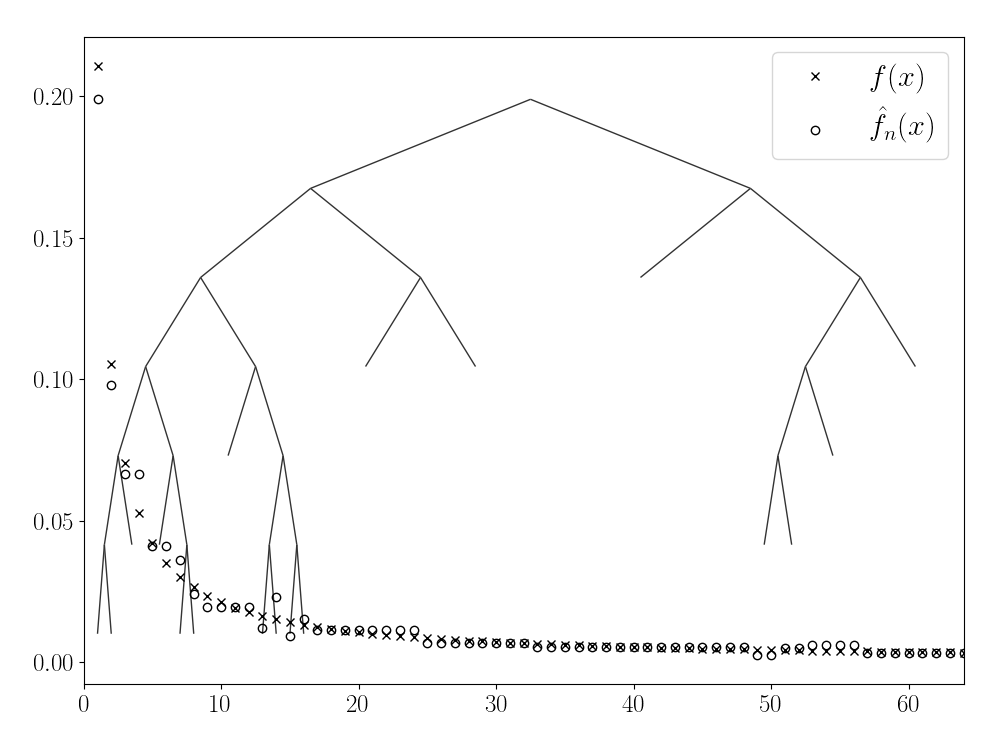
\includegraphics[width=0.85\textwidth]{n1000k64decrgreedy.png}
  \caption{One sample of $\hat{f}_n$ for $n = 1000$ and $k = 64$,
    where $f(x) = 1/(x H_k)$ for $H_k$ the $k$-th Harmonic number. The
    tree $\widehat{T}$ is overlayed.}
  \figlabel{greedy}
\end{figure}
After applying this procedure, one obtains a (random) tree
$\widehat{T}$ with leaves $\widehat{L}$, and the set
$\{I_u \colon u \in \widehat{L}\}$ forms a partition of the support
$\{1, \dots, k\}$. Let $\hat{f}_n$ be the histogram estimate based on
this partition, \ie
\[
  \hat{f}_n(x) = \frac{N_u}{n |I_u|} , \qquad \text{if $x \in I_u, u \in \widehat{L}$.}
\]
The density estimate $\hat{f}_n$ is called the \emph{greedy tree-based
  estimator}. See \figref{greedy} for a typical plot of $\hat{f}_n$,
and a visualization of the tree $\widehat{T}$.

\begin{rem}
Intuitively, we justify the rule \eqref{greedy-splitting-rule} as
follows: We expect that $N_v$ is at least as large as $N_w$ by
monotonicity of the density $f$, and the larger the difference
$|N_v - N_w|$, the finer a partition around $I_v$ and $I_w$ should be
to minimize the error of a piecewise constant estimate of
$f$. However, even if $N_v$ and $N_w$ were equal in expectation, we
expect with positive probability that $N_v$ may deviate from $N_w$ on
the order of a standard deviation, \ie on the order of
$\sqrt{N_v + N_w}$, and this determines the threshold for splitting.
\end{rem}

\begin{rem}\remlabel{birge-op}
  One could argue that any good estimate of a non-increasing density
  should itself be non-increasing, and the estimate $\hat{f}_n$ does
  not have this property. This can be rectified using a method of
  Birg\'{e}~\cite{birge-risk}, who described a transformation of
  piecewise-constant density estimates which does not increase risk
  with respect to non-increasing densities. Specifically, suppose that
  the estimate $\hat{f}_n$ is not non-increasing. Then, there are
  consecutive intervals $I_v$, $I_w$ such that $\hat{f}_n$ has
  constant value $y_v$ on $I_v$ and $y_w$ on $I_w$, and $y_v <
  y_w$. Let the transformed estimate be constant on $I_v \cup I_w$,
  with value
  \[
    \frac{y_v |I_v| + y_w |I_w|}{|I_v| + |I_w|} ,
  \]
  \ie the average value of $\hat{f}_n$ on $I_v \cup I_w$. Iterate the
  above transformation until a non-increasing estimate is obtained. It
  can be proven that this results in a unique estimate $\hat{f}_n'$,
  regardless of the order of merged intervals, and that
  \[
    \TV(\hat{f}_n', f) \le \TV(\hat{f}_n, f) .
  \]
\end{rem}

\subsection{An idealized tree-based estimator}\seclabel{ideal}

\begin{figure}
  \centering
  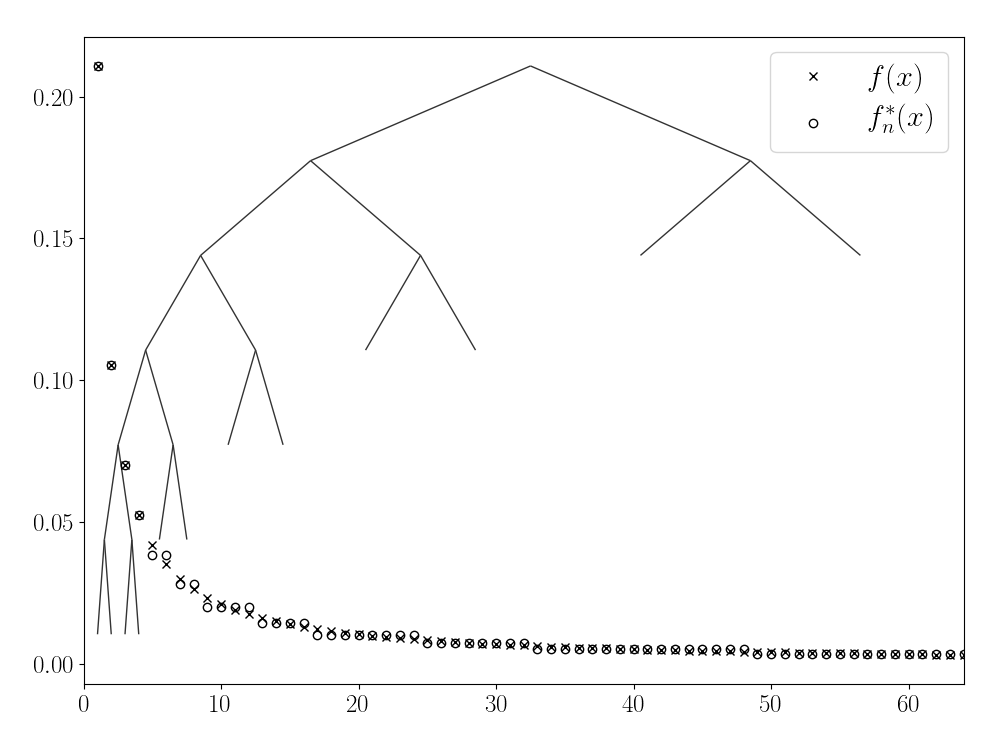
\includegraphics[width=0.85\textwidth]{n1000k64decrideal.png}
  \caption{A plot of $f^*_n$ for $n = 1000$ and $k = 64$, where
    $f(x) = 1/(x H_k)$. The tree $T^*$ is overlayed.}
  \figlabel{ideal}
\end{figure}
Instead of analyzing the greedy tree-based estimator $\hat{f}_n$ of
the preceding section, we fully analyze an idealized version.
%Indeed, we replace all of the quantities in
%\eqref{greedy-splitting-rule} with their expectations,
Indeed, in \eqref{greedy-splitting-rule}, the quantities $N_z$ are
distributed as $\Bin(n, f_z)$ for $z \in \{v, w\}$, where we define
\[
  f_z = \sum_{x \in I_z} f(x) .
\]
If we replace the quantities in \eqref{greedy-splitting-rule} with
their expectations, we obtain the \emph{idealized splitting rule}
\begin{align}
  f_v - f_w > \sqrt{\frac{f_v + f_w}{n}} , \eqlabel{id-splitting-rule}
\end{align}
where we note that $f_v \ge f_w$, since $f$ is non-increasing. Using
the same procedure as in the preceding section, replacing the
splitting rule with \eqref{id-splitting-rule}, we obtain a
deterministic tree $T^* = T^*(f)$ with leaves $L^*$, and we set
\[
  f^*_n(x) = \bar{f}_u = \frac{f_u}{|I_u|} , \qquad \text{if } x \in I_u, \, u \in L^* ,
\]
\ie $f^*_n$ is constant and equal to the average value of $f$ on each
interval $I_u$ for $u \in L^*$. We call $f^*_n$ the \emph{idealized
  tree-based estimate}. See \figref{ideal} for a visualization of
$f^*_n$ and $T^*$. It may be instructive to compare \figref{ideal} to
\figref{greedy}.

Of course, $T^*$ and $f^*_n$ both depend
intimately upon knowledge of the density $f$; in practice, we only
have access to the samples $X_1, \dots, X_n \iid f$, and the density
$f$ itself is unknown. In particular, we cannot practically use
$f^*_n$ as an estimate for unknown $f$. Importantly, as we will soon
show, we can still use $f^*_n$ along with
\corrref{minimum-distance-risk} to get a minimax rate upper bound for
$\sF_k$.

\begin{prop}\proplabel{id-tv}
  \[
    \TV(f^*_n, f) \le \frac{5}{2} \sqrt{\frac{|\{u \in L^* \colon |I_u| > 1\} |}{n}} .
  \]
\end{prop}
\begin{proof}
  Writing out the TV-distance explicitly, we have
  \begin{align*}
    \TV(f^*_n, f) &= \frac{1}{2} \sum_{x \in \{1, \dots, k\}} |f^*_n(x) - f(x)| \\
                  &= \frac{1}{2} \sum_{u \in L^*} \sum_{x \in I_u} |f^*_n(x) - f(x)| \\
                  &= \frac{1}{2} \sum_{u \in L^*} \sum_{x \in I_u} | \bar{f}_u - f(x) | .
  \end{align*}
  \begin{figure} 
    \centering
    \includegraphics{biasgraph.pdf}
    %\input{biasgraph.tex}
    \caption{A visualization of the $L_1$ distance between $f^*_n$ and
      $f$ on $I_u$.}
    \figlabel{biasarea}
  \end{figure}
  
  Let $u \in L^*$, and define
  $A_u = \sum_{x \in I_u} |\bar{f}_u - f(x)|$. If $|I_u| = 1$, then
  $A_u = 0$, so assume that $|I_u| > 1$. In this case, let $I_v$ and
  $I_w$ be the left and right halves of the interval $I_u$, and let
  $\bar{f}_v$ and $\bar{f}_w$ be the average value of $f$ on $I_v$ and
  $I_w$ respectively. Write also
  \[
    B_v = \sum_{x \in I_v} |\bar{f}_v - f(x)| , \qquad   B_w = \sum_{x \in I_w} |\bar{f}_w - f(x)| .
  \]
  Refer to \figref{biasarea}. We view $A_u$ as the positive area
  between the curve $f$ and the line $\bar{f}_u$; in the figure, this
  is the patterned area. Then, $B_v$ is the positive area between $f$
  and $\bar{f}_v$ on $I_v$, which is represented as the gray area on
  $I_v$ in \figref{biasarea}, and $B_w$ is the positive area between
  $f$ and $\bar{f}_w$ on $I_w$, the gray area on $I_w$ in
  \figref{biasarea}. For $z \in \{v, u, w\}$, let $x_z$ be the largest
  point in $I_z$ for which $f(x_z) \ge \bar{f}_z$.  By the triangle
  inequality,
  \begin{align*}
    A_u &\le (\bar{f}_v - \bar{f}_u) |I_v| + (\bar{f}_u - \bar{f}_w) |I_w| + B_v + B_w \\
        &= (f_v - f_w) + B_v + B_w .
  \end{align*}
  Furthermore,
  \begin{align*}
    B_v &= \sum_{x \in I_v, \, x \le x_v} (f(x) - \bar{f}_v) + \sum_{x \in I_v, \, x > x_v} (\bar{f}_v - f(x)) \\
        &= 2 \sum_{x \in I_v, \, x > x_v} (\bar{f}_v - f(x)) \\
        &\le 2 |I_v| (\bar{f}_v - \bar{f}_w) \\
        &= 2 (f_v - f_w) ,
  \end{align*}
  where the second equality follows by the choice of $x_v$. A similar
  relation holds for $B_w$, whence
  \[
    A_u \le 5 (f_v - f_w) \le 5 \sqrt{f_u/n} ,
  \]
  %Since the gray area on $I_v$ to the left of $x_v$ is equal to the
  %gray area on $I_v$ to the right of $x_v$, and the gray area on $I_w$
  %to the left of $x_w$ is equal to the gray area on $I_w$ to the right
  %of $x_w$, then
  %\[
  %  B_v + B_w \le (\bar{f}_v - \bar{f}_w) |I_u| .
  %\]
  %Then
  %\begin{align*}
  %  A_u &\le B_v + B_w + (\bar{f}_v - \bar{f}_w) |I_u|/2 \\
  %      &\le 3 (\bar{f}_v - \bar{f}_w) |I_u|/2 \\
  %      &= 3 (f_v - f_w) \\
  %      &\le 3 \sqrt{f_u/n} ,
  %\end{align*}
  where this last inequality follows from the splitting rule
  \eqref{id-splitting-rule}, since $u \in L^*$ and $|I_u| > 1$. So,
  \begin{align*}
    \TV(f^*_n, f) &= \frac{1}{2} \sum_{u \in L^*} A_u \\
                  &\le \frac{5}{2 \sqrt{n}} \sum_{u \in L^* \colon |I_u| > 1} \sqrt{f_u} \\
                  &\le \frac{5}{2} \sqrt{\frac{|\{u \in L^* \colon |I_u| > 1\}|}{n}} ,
  \end{align*}
  by the Cauchy-Schwarz inequality.
\end{proof}

\begin{prop}\proplabel{id-num-leaves}
  If $n \ge 64$ and $2 n^{1/3} \le k < n^{1/3} 2^n$, then
  \[
    |L^*| \le 12 n^{1/3} {\left( \log_2 (k/n^{1/3}) \right)}^{2/3} .
  \]
\end{prop}
\begin{proof}
  Note that $T^*$ has height at most $\log_2 k$. Let $U_j$ be the set
  of nodes at depth $j - 1$ in $T^*$ which have at least one leaf as a
  child, for $1 \le j \le \log_2 k$, and label the children of the
  nodes in $U_j$ in order of appeareance from right to left in $T^*$
  as $u_1, u_2, \dots, u_{2 |U_j|}$. Since none of the nodes in $U_j$
  are themselves leaves, then by \eqref{id-splitting-rule},
  \[
    f_{u_2} - f_{u_1} > \sqrt{\frac{f_{u_1} + f_{u_2}}{n} } ,
  \]
  and in particular since $f_{u_1} \ge 0$, then
  $f_{u_2} > \sqrt{f_{u_2}/n},$ so that $f_{u_2} > 1/n$. In general,
  \[
    f_{u_{2i}} > f_{u_{2i - 2}} + \sqrt{ \frac{2 f_{u_{2i - 2}}}{n} }, %\qquad \text{and} \qquad f_{u_{2i + 1}} > f_{u_{2i}} ,
  \]
  and this recurrence relation can be solved to obtain that
  \begin{align}
    f_{u_{2i}} \ge \frac{i^2}{n} . \eqlabel{monotone-leaf-prob}
  \end{align}
  Let $L_j$ be the set of leaves at level $j$ in $T^*$. The leaves at
  level $j$ in order from right to left form a subsequence
  $v_1, v_2, \dots, v_{|L_j|}$ of $u_1, u_2, \dots, u_{2|U_j|}$. Write
  $q_j$ for the total probability mass of $f$ held in the leaves
  $L_j$, \ie
  \[
    q_j = \sum_{v \in L_j} f_v = \sum_{i = 1}^{|L_j|} f_{v_i} .
  \]
  By \eqref{monotone-leaf-prob} and since $f_{v_i} \ge f_{u_i}$ for
  each $i$,
  \begin{align*}
    \sum_{i = 1}^{|L_j|} f_{v_i} \ge \sum_{i = 1}^{\floor{|L_j|/2}} f_{u_{2i}} 
                                 \ge \sum_{i = 1}^{\floor{|L_j|/2}} \frac{i^2}{n} 
                                 \ge \frac{(\floor{|L_j|/2})^3}{3 n} ,
  \end{align*}
  so that
  \[
    |L_j| \le 2 + 2(3 n q_j)^{1/3} \le 2 + 3 (n q_j)^{1/3} .
  \]
  Summing over all leaves and using the facts that $n \ge 64$ and
  $2n^{1/3} \le k < n^{1/3} 2^n$,
  \begin{align*}
    |L^*| &= \sum_{j = 0}^{\floor{(1/3) \log_2 n} - 1} |L_j| + \sum_{j = \floor{(1/3) \log_2 n}}^{\log_2 k} |L_j| \\
          &\le n^{1/3} + \sum_{j = \floor{(1/3) \log_2 n}}^{\log_2 k} (2 + 3 (n q_j)^{1/3}) \\
          &\le n^{1/3} + 4 \log_2 (k/n^{1/3}) + 3 n^{1/3} \sum_{j = \floor{(1/3) \log_2 n}}^{\log_2 k} q_{j}^{1/3} .
  \end{align*}
  By H\"{o}lder's inequality,
  \begin{align*}
    \sum_{j = \floor{(1/3) \log_2 n}}^{\log_2 k} q_{j}^{1/3} &\le {\left( \sum_{j = 1}^{\log_2 k} q_j \right)}^{1/3} {\left( \sum_{j = \floor{(1/3) \log_2 n}}^{\log_2 k} 1 \right)}^{2/3} \\
                                                                  &\le {\left(3 \log_2 (k/n^{1/3}) \right)}^{2/3} , 
  \end{align*}
  so finally
  \begin{align*}
    |L^*| &\le n^{1/3} + 4 \log_2 (k/n^{1/3}) + 7 n^{1/3} {\left( \log_2 (k/n^{1/3}) \right)}^{2/3} \\
        &\le 12 n^{1/3} {\left( \log_2 (k/n^{1/3}) \right)}^{2/3} . \qedhere
  \end{align*}
\end{proof}

\begin{proof}[Proof of the upper bound in \thmref{monotone-result}]
  The case $k \ge n^{1/3} 2^n$ is trivial, and follows simply because
  the TV-distance is always upper bounded by $1$.

  Suppose next that $2 n^{1/3} > k$. In this regime, we can use a
  histogram estimator for $f$ with bins of size $1$ for each element
  of $\{1, \dots, k\}$. It is well known that risk of this estimator
  is on the order of $\sqrt{k/n}$~\cite{comb-methods}.

  Finally, suppose that $2 n^{1/3} \le k < n^{1/3} 2^n$. Let
  $\sF_\Theta$ be the class of all piecewise-constant probability
  densities on $\{1, \dots, k\}$ which have $\ell = |L^*|$ parts; in
  particular, $f^*_n \in \sF_\Theta$. Let $\sA_\Theta$ be the Yatracos
  class of $\sF_\Theta$,
  \[
    \sA_\Theta = \Bigl\{ \{x \colon f(x) > g(x)\} \colon f \neq g \in \sF_\Theta\Bigr\} .
  \]
  Then, $\sA_\Theta \subseteq \sA$, where $\sA$ is the class of all
  unions of at most $\ell$ intervals in $\N$. It is well known that
  $\VC(\sA) = 2\ell$, so $\VC(\sA_\Theta) \le 2\ell$. By
  \corrref{minimum-distance-risk} and \propref{id-tv}, there are
  universal constants $c_1, c_2 > 0$ for which
  \begin{align*}
    \sR_n(\sF_k) &\le 3 \sup_{f \in \sF_k} \inf_{\theta \in \Theta} \TV(f_{n, \theta}, f) + c_1 \sqrt{\ell/n} \\
                 &\le 3 \sup_{f \in \sF_k} \TV(f^*_n, f) + c_1 \sqrt{\ell/n} \\
                 &\le c_2 \sqrt{\ell/n} .
  \end{align*}
  By \propref{id-num-leaves}, we see that for sufficiently large $n$,
  there is a universal constant $c_3 > 0$ such that
  \[
    \sR_n(\sF_k) \le c_3 {\left( \frac{\log (k/n^{1/3})}{n} \right)}^{1/3} . \qedhere
  \]
\end{proof}

\begin{rem}\remlabel{cont-monotone}
  Fix $B > 0$ and let $\sF_B'$ be the class of all non-increasing
  densities supported on $[0, 1]$ and bounded from above by $B$. Our
  method can be applied to prove a minimax rate upper bound
  $\sF_B'$. Now, the tree $T^*$ underlying the idealized tree-based
  estimator is truncated at some given level, say $m$ to be specified,
  and the idealized estimator should take on the average value of the
  true density $f$ on the truncated leaves. Write $d(u)$ for the depth
  of the node $u$ in $T^*$. As in \propref{id-tv},
  \begin{align*}
    &\TV(f_n^*, f) = \frac{1}{2} \sum_{u \in L^*} A_u \\
    & \qquad\le \frac{5}{2 \sqrt{n}} \sum_{u \in L^*, \, d(u) < m} \sqrt{f_u} + \frac{1}{2} \sum_{u \in L^*, \, d(u) = m} A_u .
  \end{align*}
  The argument of \propref{id-num-leaves} allows us to control the
  first sum, so that for some universal constant $c_1 > 0$,
  \[
    \frac{5}{2\sqrt{n}} \sum_{u \in L^*, \, d(u) < m} \sqrt{f_u} \le c_1 {\left( \frac{m}{n}\right)}^{1/3} .
  \]
  On the other hand, since $A_u \le 5(f_v - f_w)$ for $v$ the left
  child and $w$ the right child of $u$, then
  \[
    \frac{1}{2} \sum_{u \in L^*, \, d(u) = m} A_u \le \frac{5 B}{2^{m + 2}} .
  \]
  An optimal choice of $m$ has that for a universal constant
  $c_2 > 0$,
  \[
    \TV(f_n^*, f) \le c_2 {\left(\frac{\log_2 (B n^{1/3})}{n}\right)}^{1/3} .
  \]
  From here, using the same method as in the proof of
  \thmref{monotone-result}, it follows that for some universal
  $c_3 > 0$,
  \[
    \sR_n(\sF_B') \le c_3 {\left(\frac{\log_2 (B
          n^{1/3})}{n}\right)}^{1/3} .
  \]
\end{rem}
